\section{Methods}
In this paper, three different probablistic formulations exist for the underlying edge importance model. All three of these models rely upon the excellent \verb|Pyro| \cite{bingham_pyro_2018} framework for implementation and inference. Additionally, all GNN models are trained through the \verb|pytorch_geometric| \cite{fey_fast_2019} and \verb|pytorch| \cite{paszke_pytorch_2019} frameworks.

\subsection{Beta Model}
The first method used in this paper is a prior in which all Beta distributions are considered independent of each other. Specifically, we assume that $\mathcal{E}_i = E$ and that
\begin{align*}
	\mathcal{W}_i = \{\mathcal{W}_i(v_j , v_k) \mid (v,j, v_k) \in E\}
\end{align*}
with
\begin{align*}
	\mathcal{W}_i(v_j, v_k) = \mathbb{E}[Beta(\alpha_{j}, \beta_{k})]
\end{align*}
with $Beta(\alpha_{j,k}, \beta_{j, k})$ representing the prior Beta distribution on edge $(v_j, v_k)$ with specific parameters $\alpha_{j,k}$ and $\beta_{j,k}$. Note, we define the Beta distribution as
\begin{align*}
	\mathcal{P}(Beta(\alpha, \beta) = x) &= \frac{x^{\alpha - 1}(1-x)^{\beta - 1}}{\Beta(\alpha, \beta)} \\
	\Beta(\alpha, \beta) &= \frac{\Gamma(\alpha)\Gamma(\beta)}{\Gamma(\alpha + \beta)}
\end{align*}
where $\Gamma$ is the canoncical Gamma function \cite{noauthor_continuous_nodate}. Given this, the goal of the interpretation task is to learn a variational family $q_{\phi}(H)$ that most closely resembles the posterior distribution when the categorical distribution
\begin{align*}
	\phi(v_i, \mathcal{X}, E, \mathcal{W}_i)
\end{align*}
is conditioned on the full model
\begin{align*}
	\phi(v_i, \mathcal{X}, E, \mathcal{W})
\end{align*}
where $\mathcal{W}(e) = 1$ for all $e \in E$. For the sake of this experiment, the posterior distribution is also assumed to be a set of Beta distributions but fully conditional on each other. The goal, then is to learn posterior values $\hat{\alpha}_{j,k}$ and $\hat{\beta}_{j,k}$. Given these values, the final explanation is
\begin{align*}
	\mathcal{W}_i(v_j, v_k) = \mathbb{E}[Beta(\hat{\alpha}_{j}, \hat{\beta}_{k})]
\end{align*}
which has an easily derived closed form.

\subsubsection{Interpretation of the Beta Model}
\begin{figure}[t]
	\centering
	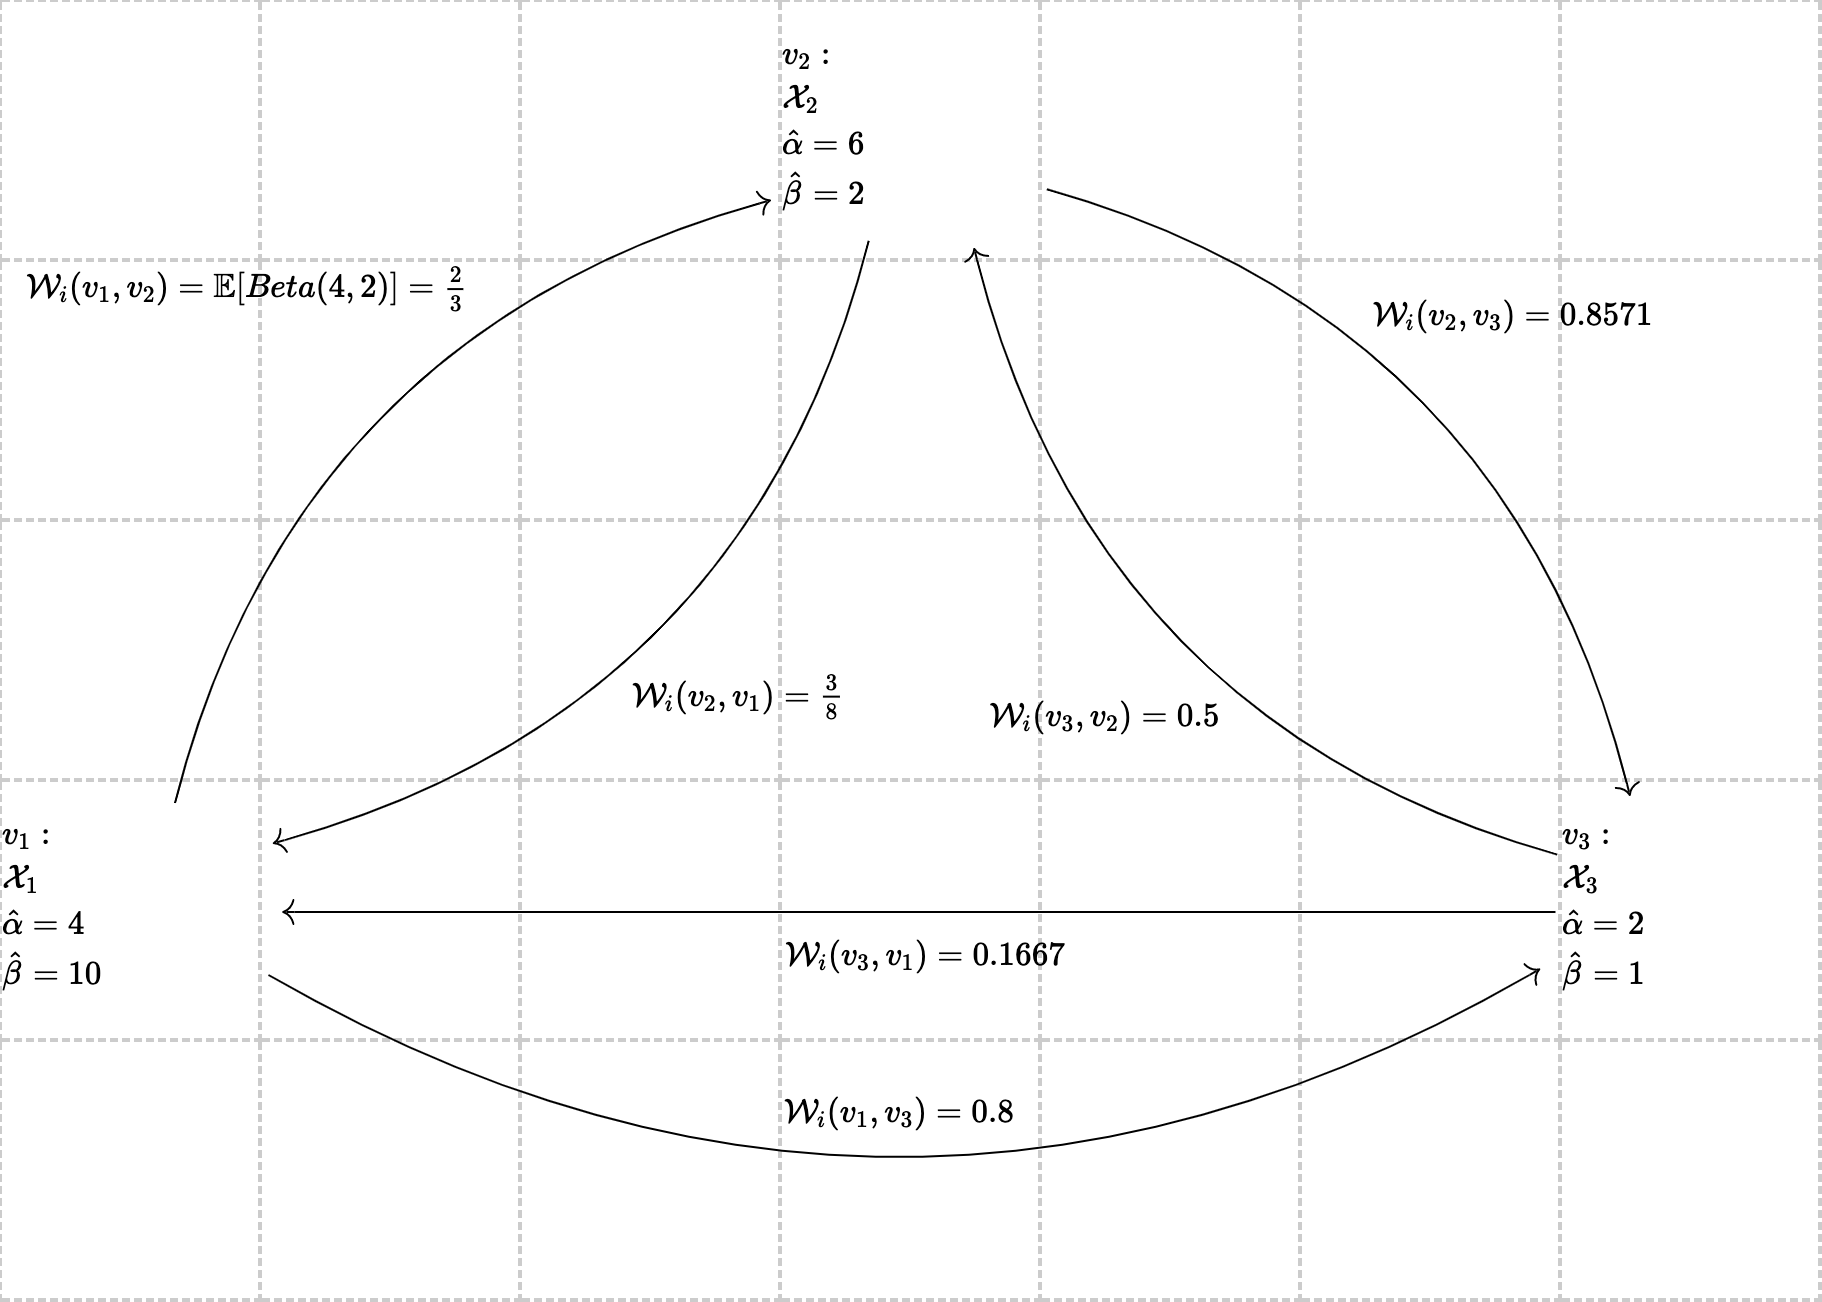
\includegraphics[width=\textwidth]{images/beta_ex.png}
	\caption{An example of a Beta posterior that shows information flowing from $v_1$ to $v_3$.}
	\label{fig:beta-ex}
\end{figure}
There is a wide array of literature on the use of Exponential-families for the modeling of edge weight priors. In particular, the work of Bolla \cite{bolla_estimating_2017} is important. In this work, edge weights are modeled by conditionally independent Beta distributions. The parameters of these Beta distributions are updated via a closed-form solution but it serves as a good model for prediction propogation of information or material from one node to another and converging on a steady-state for the propogation. In the case of GNNs, one can imagine the \verb|MSG| operation as the sending of information. The dense layers in the \verb|Upd| step, then, learn the weight to assign to each incoming and outgoing message. In this vein, the Beta model can approximate this "attention" that is paid in the \verb|Upd| step. Hence, the goal of this model is to serve as an approximiation of this process and encode the steady-state flow of information in the model.
\begin{figure}[t]
	\centering
	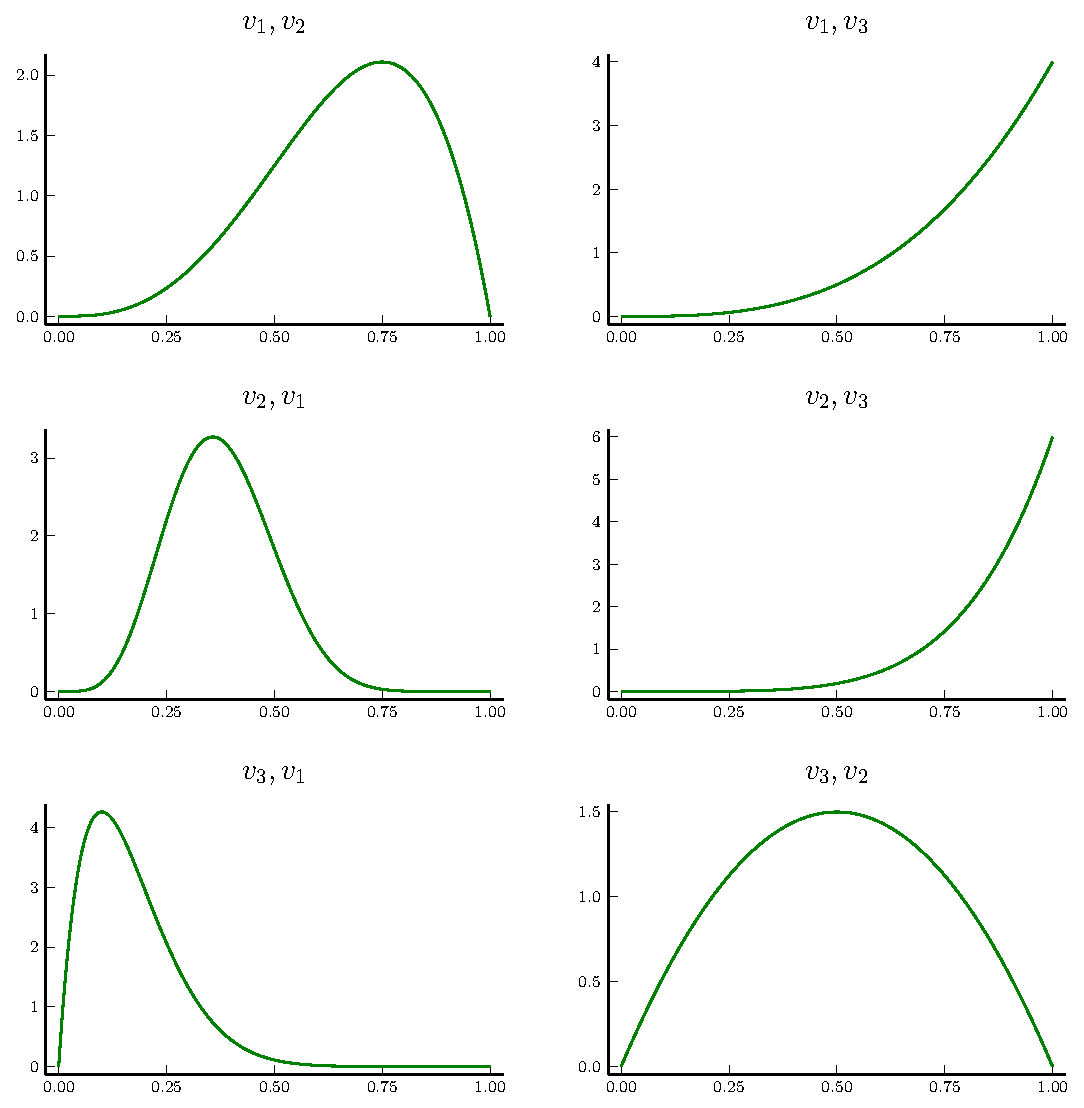
\includegraphics[width=0.8\textwidth]{images/beta_post.pdf}
	\caption{Posterior distributions for each edge in \ref{fig:beta-ex}}
	\label{fig:beta-ex-post}
\end{figure}

In this model, the $\alpha$ values serve to desribe the affinity for information to flow out of a node while the $\beta$ values tend to describe the affinity for information to flow into the node. Together, they describe the steady state flow of information and perfectly describe many networks in which pathways of information lead to end-goal expression. Indeed, since GNNs tend to embed this type of information flow in a deep-learning setting, it serves to reason that such a prior would be a good encapsulation of the process of information flow, especially at steady state. A typical example of this is gene expression in biology \cite{petralia_new_2016} where paths of edges represent regulatory pathways directly. 

An example of this flow can be seen in figure \ref{fig:beta-ex}. In this figure, we consider a hypothetical posterior for this model and demonstrate how it describes the flow of information from node $v_1$ to $v_3$ via these $\alpha$ and $\beta$ parameters. Additionally, in figure \ref{fig:beta-ex-post}, one can see the posterior distribution of each edge. Notably, there is no conditional independence in this model as changing the parameter on one node changes all adjoining edges.